\AdvanceDate[0]

\begin{document}
\pagestyle{fancy}
\fancyhead[L]{Seconde 13}
\fancyhead[C]{\textbf{Probabilités 2 \ifsolutions -- Solutions  \fi}}
\fancyhead[R]{\today}

\exe{	
	On tire un boule dans une urne contenant $2$ boules rouges et $4$ boules vertes.
	\begin{enumerate}[label=$\bullet$]
		\item Si la boule tirée est verte, on la met de côté et on retire une nouvelle boule
		\item Si la boule tirée est rouge, on la remet dans l'urne et on retire une nouvelle boule
	\end{enumerate}
	On distingue les quatre événements suivants :
		\begin{multicols}{2}
		\begin{enumerate}[label=]
			\item v : \og la première boule tirée est verte \fg
			\item r : \og la première boule tirée est rouge \fg
			\item V : \og la deuxième boule tirée est verte \fg
			\item R : \og la deuxième boule tirée est rouge \fg
		\end{enumerate}
		\end{multicols}
	\begin{center}
	\begin{tikzpicture}
		% depth 1
		\foreach \i in {-3, 3}
		\draw[-, thick, black] (0,0) node {$\bullet$} -- (\i,-2);
		% depth 2
		\foreach \i in {-3, 3} \foreach \j in {-1, 1}
			\draw[-, thick, black] (\i,-2) node {$\bullet$} -- (\i+\j,-4) node {$\bullet$};
			
		\draw (-3,-2) node[above left] {v};
		\draw (3,-2) node[above right] {r};
			
		\draw (-4,-4) node[below] {V};
		\draw (2,-4) node[below] {V};
		\draw (-2,-4) node[below] {R};
		\draw (4,-4) node[below] {R};
	\end{tikzpicture}
	\end{center}
	Compléter l'arbre, et calculer $P(V)$ et $P(R)$.
}{
	\, \\
	\begin{center}
	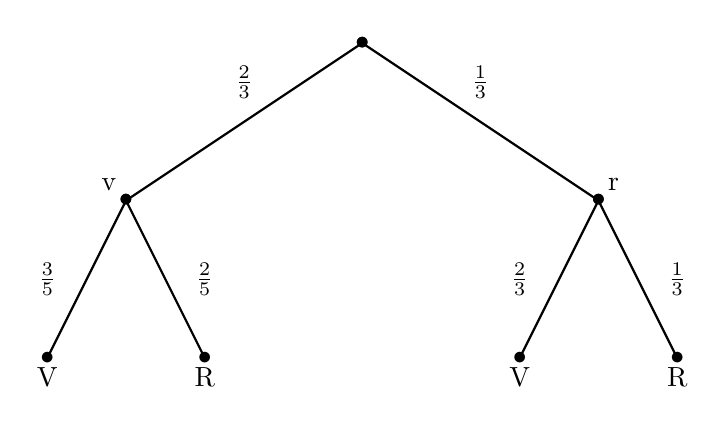
\begin{tikzpicture}
		% depth 1
		\foreach \i in {-3, 3}
		\draw[-, thick, black] (0,0) node {$\bullet$} -- (\i,-2);
		% depth 2
		\foreach \i in {-3, 3} \foreach \j in {-1, 1}
			\draw[-, thick, black] (\i,-2) node {$\bullet$} -- (\i+\j,-4) node {$\bullet$};
			
		\draw (-3,-2) node[above left] {v};
		\draw (3,-2) node[above right] {r};
			
		\draw (-4,-4) node[below] {V};
		\draw (2,-4) node[below] {V};
		\draw (-2,-4) node[below] {R};
		\draw (4,-4) node[below] {R};
		
		% sols
		\draw (1.5,-.5) node {$\frac13$};
		\draw (-1.5,-.5) node {$\frac23$};
		
		\draw (4,-3) node {$\frac13$};
		\draw (2,-3) node {$\frac23$};
		
		\draw (-2,-3) node {$\frac25$};
		\draw (-4,-3) node {$\frac35$};
	\end{tikzpicture}
	\end{center}
	La probabilité d'une issue est la somme des probabilités de chacun des chemins racine-feuille.
	Pour obtenir la probabilité d'un chemin racine-feuille, on multiplie les probabilités rencontrées en le parcourant.
	
		\begin{align*}
			P(V) &= \dfrac23 \times \dfrac35 + \dfrac13 \times \dfrac23 \\
				&= \dfrac25 + \dfrac29 \\
				&= \dfrac{18 + 10}{5 \times 9} = \dfrac{28}{45}
		\end{align*}
	
		\begin{align*}
			P(R) &= \dfrac23 \times \dfrac25 + \dfrac13 \times \dfrac13 \\
				&= \dfrac4{15} + \dfrac19 \\
				&= \dfrac{36 + 15}{15 \times 9} = \dfrac{51}{135} = \dfrac{17}{45}
		\end{align*}
		
		On aurait aussi pû utiliser le fait que $P(R) = 1 - P(V)$ pour ne pas augmenter la probabilité de faire une erreur de calcul.
}


\exe{
	Compléter l'arbre correspondant à une expérience aléatoire à deux épreuves d'univers $\{A ; B ; C ; D\}$ et répondre aux questions suivantes.
	\begin{center}
	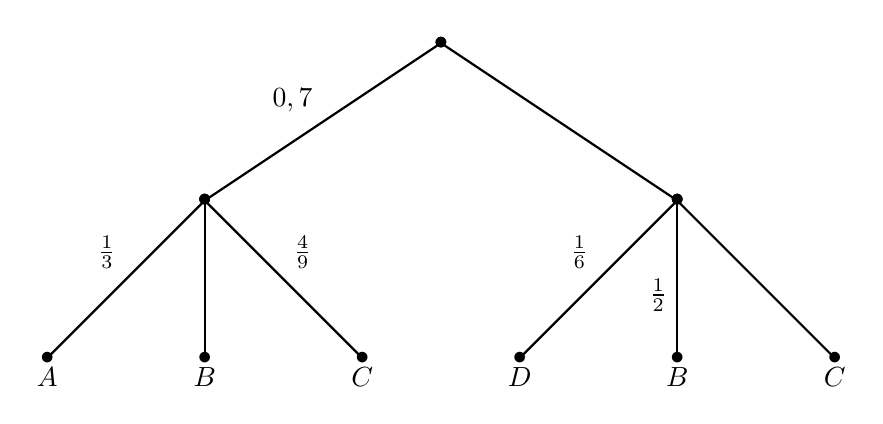
\begin{tikzpicture}
		% depth 1
		\draw[-, thick, black] (0,0) node {$\bullet$} -- (3,-2) node[midway, above right] {};
		\draw[-, thick, black] (0,0) node {$\bullet$} -- (-3,-2) node[midway, above left] {$0,7$};
		% depth 2
		\draw[-, thick, black] (-3,-2) node {$\bullet$} -- (-1,-4) node[midway, above right] {$\frac49$};
		\draw[-, thick, black] (-3,-2) node {$\bullet$} -- (-3,-4);
		\draw[-, thick, black] (-3,-2) node {$\bullet$} -- (-5,-4) node[midway, above left] {$\frac13$};
		
		\draw[-, thick, black] (3,-2) node {$\bullet$} -- (1,-4) node[midway, above left] {$\frac16$};
		\draw[-, thick, black] (3,-2) node {$\bullet$} -- (3,-4) node[pos=.6, left] {$\frac12$};
		\draw[-, thick, black] (3,-2) node {$\bullet$} -- (5,-4);
		
		\draw (1,-4) node {$\bullet$};
		\draw (3,-4) node {$\bullet$};
		\draw (5,-4) node {$\bullet$};
		\draw (1,-4) node[below] {$D$};
		\draw (3,-4) node[below] {$B$};
		\draw (5,-4) node[below] {$C$};
		
		\draw (-1,-4) node {$\bullet$};
		\draw (-3,-4) node {$\bullet$};
		\draw (-5,-4) node {$\bullet$};
		\draw (-1,-4) node[below] {$C$};
		\draw (-3,-4) node[below] {$B$};
		\draw (-5,-4) node[below] {$A$};
	\end{tikzpicture}
	\end{center}
	
	\begin{multicols}{2}
	\begin{enumerate}
		\item Calculer $P(D)$.
		\item Calculer $P(B)$.
		\item Calculer $P(D \cup B)$.
		\item Calculer $P(A\cup C)$.
	\end{enumerate}
	\end{multicols}

}{
	La somme des probabilités de chaque sous-branche est toujours $1$. 
	On complète donc l'arbre comme ci-dessous.
	
	\begin{center}
	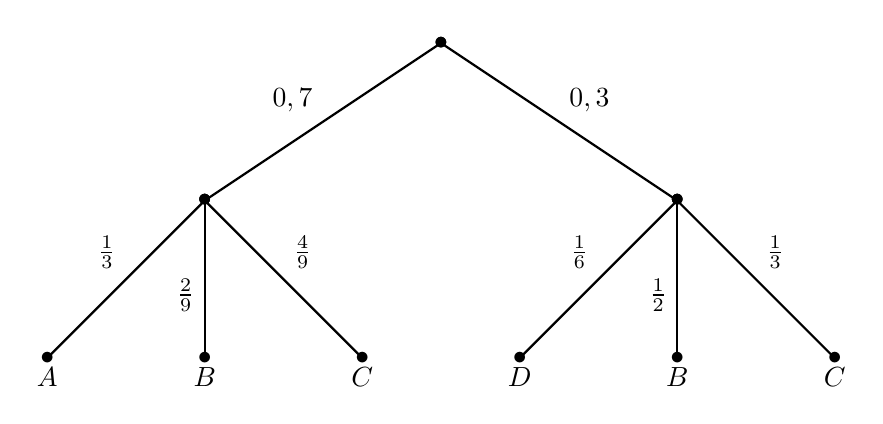
\begin{tikzpicture}
		% depth 1
		\draw[-, thick, black] (0,0) node {$\bullet$} -- (3,-2) node[midway, above right] {$0,3$};
		\draw[-, thick, black] (0,0) node {$\bullet$} -- (-3,-2) node[midway, above left] {$0,7$};
		% depth 2
		\draw[-, thick, black] (-3,-2) node {$\bullet$} -- (-1,-4) node[midway, above right] {$\frac49$};
		\draw[-, thick, black] (-3,-2) node {$\bullet$} -- (-3,-4) node[pos=.6, left] {$\frac29$};
		\draw[-, thick, black] (-3,-2) node {$\bullet$} -- (-5,-4) node[midway, above left] {$\frac13$};
		
		\draw[-, thick, black] (3,-2) node {$\bullet$} -- (1,-4) node[midway, above left] {$\frac16$};
		\draw[-, thick, black] (3,-2) node {$\bullet$} -- (3,-4) node[pos=.6, left] {$\frac12$};
		\draw[-, thick, black] (3,-2) node {$\bullet$} -- (5,-4) node[midway, above right] {$\frac13$};
		
		\draw (1,-4) node {$\bullet$};
		\draw (3,-4) node {$\bullet$};
		\draw (5,-4) node {$\bullet$};
		\draw (1,-4) node[below] {$D$};
		\draw (3,-4) node[below] {$B$};
		\draw (5,-4) node[below] {$C$};
		
		\draw (-1,-4) node {$\bullet$};
		\draw (-3,-4) node {$\bullet$};
		\draw (-5,-4) node {$\bullet$};
		\draw (-1,-4) node[below] {$C$};
		\draw (-3,-4) node[below] {$B$};
		\draw (-5,-4) node[below] {$A$};
	\end{tikzpicture}
	\end{center}
	
	\begin{enumerate}
		\item 
			\begin{align*}
				P(D) &= 0,3 \times \dfrac16 \\ &= \dfrac{0,3}{6} \\ &= \dfrac{0,1}{2} = 0,05.
			\end{align*}
		\item 
			\begin{align*}
				P(B) &= 0,7 \times \dfrac29 + 0,3 \times \dfrac12 \approx 0,31.
			\end{align*}
		\item 
			Comme $D$ et $B$ sont deux issues distinctes de l'univers, on a
			\begin{align*}
				P(D \cup B) &= P(D) + P(B) \\ &\approx 0,05 + 0,31 = 0,36.
			\end{align*}
		\item On peut soit procéder comme ci-dessus, ou alors utiliser le fait que
			\[ P(A\cup C) = P(A) + P(C) = 1 - \left( P(D) + P(B) \right) = 1 - P(D \cup B), \]
		et donc
			\[ P(A\cup C) \approx 0,64. \]
	\end{enumerate}
}

\newpage

\exe{
	On tire un boule dans une urne contenant $3$ boules bleues et $4$ boules vertes.
	\begin{enumerate}[label=$\bullet$]
		\item Si la boule tirée est verte, on jette un dé équilibré à $3$ faces
		\item Si la boule tirée est bleue, on jette un dé équilibré à $6$ faces
	\end{enumerate}

	Créer un arbre de probabilité pour cette situation et répondre aux questions suivantes.
	\begin{enumerate}
		\item Quelle est la probabilité d'obtenir un nombre pair ?
		\item Quelle est la probabilité d'obtenir un multiple de $3$ ?
		\item Quelle est la probabilité d'obtenir un nombre pair \textbf{ou} un multiple de $3$ ?
		\item Calculer la probabilité d'obtenir $6$ et vérifier la formule d'inclusion-exclusion.
	\end{enumerate}

}{
	On a l'arbre suivant.
	
	\begin{center}
	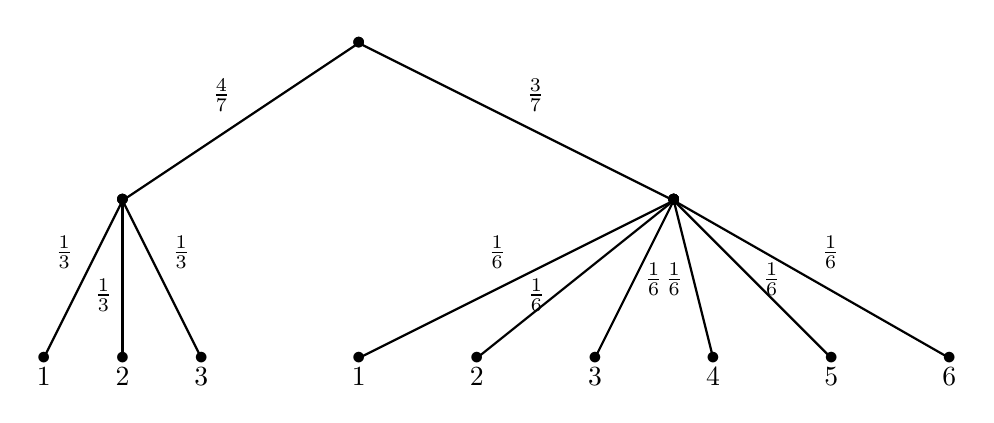
\begin{tikzpicture}
		% depth 1
		\draw[-, thick, black] (0,0) node {$\bullet$} -- (4,-2) node[midway, above right] {$\frac37$};
		\draw[-, thick, black] (0,0) node {$\bullet$} -- (-3,-2) node[midway, above left] {$\frac47$};
		% depth 2
		% gauche -> droite
		% verte
		\draw[-, thick, black] (-3,-2) node {$\bullet$} -- (-2,-4) node[midway, above right] {$\frac13$};
		\draw[-, thick, black] (-3,-2) node {$\bullet$} -- (-3,-4) node[pos=.6, left] {$\frac13$};
		\draw[-, thick, black] (-3,-2) node {$\bullet$} -- (-4,-4) node[midway, above left] {$\frac13$};
		
		\draw (-4,-4) node {$\bullet$};
		\draw (-3,-4) node {$\bullet$};
		\draw (-2,-4) node {$\bullet$};
		\draw (-4,-4) node[below] {$1$};
		\draw (-3,-4) node[below] {$2$};
		\draw (-2,-4) node[below] {$3$};
		
		% bleue
		\draw[-, thick, black] (4,-2) node {$\bullet$} -- (0,-4) node[midway, above left] {$\frac16$};
		\draw[-, thick, black] (4,-2) node {$\bullet$} -- (1.5,-4) node[pos=.6, left] {$\frac16$};
		\draw[-, thick, black] (4,-2) node {$\bullet$} -- (3,-4) node[midway, right] {$\frac16$};
		\draw[-, thick, black] (4,-2) node {$\bullet$} -- (4.5,-4) node[midway, left] {$\frac16$};
		\draw[-, thick, black] (4,-2) node {$\bullet$} -- (6,-4) node[midway, right] {$\frac16$};
		\draw[-, thick, black] (4,-2) node {$\bullet$} -- (7.5,-4) node[midway, above right] {$\frac16$};
		
		\draw (0,-4) node {$\bullet$};
		\draw (1.5,-4) node {$\bullet$};
		\draw (3,-4) node {$\bullet$};
		\draw (4.5,-4) node {$\bullet$};
		\draw (6,-4) node {$\bullet$};
		\draw (7.5,-4) node {$\bullet$};
		\draw (0,-4) node[below] {$1$};
		\draw (1.5,-4) node[below] {$2$};
		\draw (3,-4) node[below] {$3$};
		\draw (4.5,-4) node[below] {$4$};
		\draw (6,-4) node[below] {$5$};
		\draw (7.5,-4) node[below] {$6$};
		
	\end{tikzpicture}
	\end{center}
	
	\begin{enumerate}
		\item
			\begin{align*}
				P(\text{\og nombre pair \fg}) &= P(2) + P(4) + P(6) \\
					&= \left( \dfrac47 \times \dfrac13 + \dfrac37\times\dfrac16 \right) + \left( \dfrac37 \times \dfrac16 \right) + \left( \dfrac37 \times \dfrac16 \right) \\
					&= \dfrac4{21} + \dfrac1{14} + \dfrac1{14} + \dfrac1{14} \\
					&= \dfrac{17}{42}.
			\end{align*}
		\item
			\begin{align*}
				P(\text{\og multiple de $3$ \fg}) &= P(3) + P(6) \\
					&= \left( \dfrac47 \times \dfrac13 + \dfrac37\times\dfrac16 \right) + \left( \dfrac37 \times \dfrac16 \right) \\
					&= \dfrac4{21} + \dfrac1{14} + \dfrac1{14} \\
					&= \dfrac13.
			\end{align*}
		\item
			\begin{align*}
				P(\text{\og multiple de $3$ ou de $2$ \fg}) &= P(2) + P(3) + P(4) + P(6) \\
					&= \left( \dfrac47 \times \dfrac13 + \dfrac37\times\dfrac16 \right) + \left( \dfrac47 \times \dfrac13 + \dfrac37\times\dfrac16 \right) + \left( \dfrac37 \times \dfrac16 \right) + \left( \dfrac37 \times \dfrac16 \right) \\
					&= \dfrac4{21} + \dfrac1{14} + \dfrac4{21} + \dfrac1{14} + \dfrac1{14} + \dfrac1{14} \\
					&= \dfrac23.
			\end{align*}
		\item 
			\begin{align*}
				P(6) &=\left( \dfrac37 \times \dfrac16 \right) \\
					&= \dfrac1{14}.
			\end{align*}
			
		On vérifie l'inclusion-exclusion en comparant $P(\text{\og multiple de $3$ ou de $2$ \fg})$ et $P(\text{\og multiple de $3$ \fg}) + P(\text{\og multiple de $2$ \fg}) - P(6)$.
		D'une part,
			\[ P(\text{\og multiple de $3$ ou de $2$ \fg}) = \dfrac23, \]
		et d'autre part,
			\begin{align*}
				P(\text{\og multiple de $3$ \fg}) + P(\text{\og multiple de $2$ \fg}) - P(6) &= \dfrac13 + \dfrac{17}{42} - \dfrac1{14} \\
				&= \dfrac{14 + 17 - 3}{42} \\
				&= \dfrac{28}{42} = \dfrac23.
			\end{align*}
	\end{enumerate}
}

\exe{	
	Dans une urne opaque se trouvent un nombre inconnu de boules rouges, bleues, et vertes.
	On tire aléatoirement une boule de l'urne, on note sa couleur, et on la remet dans l'urne.
	Les résultats sont décrits dans le tableau suivant.
	\begin{center}
	\begin{tabular}{|c|c|c|c|} \hline
		Couleur & Rouge & Bleu & Vert \\ \hline
		Nombre de tirages & \rouge & \bleu & \vert \\ \hline
		Fréquence & \ifsolutions $\color{red} 0,33$ \fi  & \ifsolutions $\color{red} 0,50$ \fi & \ifsolutions $\color{red} 0,16$ \fi \\ \hline
	\end{tabular}
	\end{center}
	
	Compléter le tableau, modéliser la réalité en définissant un univers et une loi de probabilité, et l'utiliser pour répondre aux questions suivantes.
	\begin{enumerate}
		\item Quelle est la probabilité d'obtenir deux boules rouges en deux tirages ?
		\item Quelle est la probabilité d'obtenir deux boules vertes en trois tirages ?
		\item Quelle est la probabilité d'obtenir au moins une boule bleue en quatre tirages ?
	\end{enumerate}
}{
	Les fréquences sont calculées à $10^{-2}$ près dans le tableau de l'énoncé.
	On modélise la réalité en assignant les probabilités suivantes.
		\begin{align*}
			P(\text{Rouge}) = \dfrac13 && P(\text{Bleu}) = \dfrac12 && P(\text{Vert}) = \dfrac16
		\end{align*}
	On vérifie bien sûr que la somme fasse bien $1$ : $\dfrac13 + \dfrac12 + \dfrac16 = 1$.

	\begin{enumerate}
		\item 
			On crée un arbre binaire de profondeur $2$ à deux événements : $E$ et $\overline{E}$ où
				\begin{center}
					E : \og tirer une boule rouge \fg.
				\end{center}
			On en déduit que
			\[ P(\text{deux boules rouges en deux tirages}) = \dfrac13 \times \dfrac13 = \dfrac19. \]
		\item 
			On crée un arbre binaire de profondeur $3$ à deux événements : $F$ et $\overline{F}$ où
				\begin{center}
					F : \og tirer une boule verte \fg.
				\end{center}
			On lit trois issues possibles pour l'événement : $FF\overline{F}$, $F\overline{F}F$, et $\overline{F}FF$.
			Chaque issue a probabilité $\dfrac16 \times \dfrac16 = \dfrac1{36}$, donc
			\[ P(\text{deux boules vertes en trois tirages}) = 3\times \dfrac1{36} = \dfrac1{12}. \]
		\item Quelle est la probabilité d'obtenir au moins une boule bleue en quatre tirages ?
			On crée un arbre binaire de profondeur $4$ à deux événements : $G$ et $\overline{G}$ où
				\begin{center}
					G : \og tirer une boule bleue \fg.
				\end{center}
			On lit une seule issue pour l'événement complémentaire, et donc
			\[ P(\text{aucune boule bleue en quatre tirages}) = \dfrac12\times\dfrac12\times\dfrac12\times\dfrac12= \dfrac{1}{16}. \]
			Par conséquent, 
			\[ P(\text{au moins une boule bleue en quatre tirages}) =1- \dfrac{1}{16} = \dfrac{15}{16} = 0,9375. \]
	\end{enumerate}
}

\exe{	
	On lance un grand nombre de fois un D$6$, dé à $6$ faces.
	Les résultats sont décrits dans le tableau suivant.
	\begin{center}
	\begin{tabular}{|c|c|c|c|c|c|c|} \hline
		Face & 1 & 2 & 3 & 4 & 5 & 6 \\ \hline
		Nombre de tirages & \un & \deux & \trois & \quatre & \cinq & \six \\ \hline
		Fréquence & \ifsolutions $\color{red} 0,2$ \fi & \ifsolutions $\color{red} 0,3$ \fi & \ifsolutions $\color{red} 0,1$ \fi & \ifsolutions $\color{red} 0,15$ \fi & \ifsolutions $\color{red} 0,2$ \fi & \ifsolutions $\color{red} 0,05$ \fi \\ \hline
	\end{tabular}
	\end{center}
	
	Compléter le tableau, modéliser la réalité en définissant un univers et une loi de probabilité, et l'utiliser pour répondre aux questions suivantes.
	\begin{enumerate}
		\item Quelle est la probabilité d'obtenir un nombre pair ?
		\item Quelle est la probabilité d'obtenir deux $6$ en deux lancers consécutifs ?
		\item Quelle est la probabilité d'obtenir au moins un $6$ après $4$ lancers ?
	\end{enumerate}
}{
	Les fréquences sont calculées à $10^{-2}$ près dans le tableau de l'énoncé.
	On modélise la réalité en assignant les probabilités suivantes.
		\begin{align*}
			P(1) = \dfrac15 && P(2) = \dfrac3{10} && P(3) = \dfrac1{10} && P(4) = \dfrac3{20} && P(5) = \dfrac15 && P(6) = \dfrac1{20}
		\end{align*}
	On s'assure bien que la somme soit $1$ : 
		\[ \dfrac15 + \dfrac3{10} + \dfrac1{10} + \dfrac3{20} + \dfrac15 + \dfrac1{20} = \dfrac{4+6+2+3+4+1}{20} = 1. \]
	
	\begin{enumerate}
		\item 
			\begin{align*}
				P(\text{\og obtenir un nombre pair \fg}) &= P(2) + P(4) + P(6) \\
				&= 0,3 + 0,15 + 0,05 \\
				&= 0,4 = \frac25.
			\end{align*}
		\item
			On crée un arbre binaire de profondeur $2$ à deux événements : $E$ et $\overline{E}$ où
				\begin{center}
					E : \og obtenir $6$ \fg.
				\end{center}
			On en déduit que
			\[ P(\text{deux $6$ en deux lancers}) = 0,05 \times 0,05 = \left(\dfrac1{20}\right)^2 = \dfrac1{400} = 0,0025. \]
		\item
			On complète l'arbre binaire de la question précédente pour qu'il atteigne une profondeur $4$.
			L'événement complémentaire correspond à une unique issue, de probabilité
				\[ P(\text{aucun $6$ en $4$ lancers}) = 0.95^4 = \left(\dfrac{19}{20}\right)^4 = \dfrac{19^4}{20^4} = \dfrac{130321}{160000} \approx 0,81. \]
			On conclut donc que
				\[ P(\text{au moins un $6$ en $4$ lancers}) = 1-0.95^4 \approx 0,19. \]
				
	\end{enumerate}
}

\end{document}
